\chapter{Results}
This part of the document contains all the neccessary information about the cracking done in given exercises.
The cracking exercises are organized by domains, with each domain representing a specific testing environment. Each issue is described in detail, 
including its basic information, minimal proof of concept.

% region domain 1 

\section{Subdomain 1}
\textbf{Platform}: TIM environment\\
\textbf{Server IP address}: 193.167.189.112

\subsection{Password cracking with John the Ripper and Hashcat} \label{ss: issue-1}
In this exercise, i performed password cracking utilizing two popular tools: John the Ripper and Hashcat. 
The goal was to identify weak passwords and usernames that could potentially be exploited by "attackers".

Usernames and passwords were obtained from the TIM environment, and both tools were tested 
to perform the cracking process.

Usernames found: anna, riku
Passwords found: airborne, columbia3

\subsubsection{Minimal proof of concept}
Gerenal step:
I started the exercise by figuring out where the passwords were located. It was found at
\begin{verbatim} /usr/share/common_3k.txt \end{verbatim}

John the Ripper: \\
I used unshadowing technique to prepare the password file for cracking, called the file "myfile". 
The command i used was: 
\begin{verbatim}
unshadow /etc/passwd.kybs2004 /etc/shadow.kybs2004 > myfile
\end{verbatim}
where passwd and shadow files were located at /etc directory.

With this i could start the cracking process with John the Ripper. \\ 
For the task i had to figure out from the rules what rules i wanted to use.
For the first cracking process i used no flags with the command: 
\begin{verbatim}
john --wordlist=/usr/share/common_3k.txt myfile
\end{verbatim}
which resulted in finding the password "airborne" for user "anna". \\
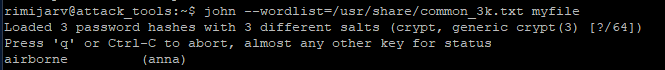
\includegraphics{anna.png}

For the second cracking process i used the flag "--rules" which added some rules to the cracking process.
In particular we wanted to use [0-9] rule which adds digits to the end of the password.
The command i used was:
\begin{verbatim}
john --wordlist=/usr/share/common_3k.txt --rules myfile
\end{verbatim}
which resulted in finding the password "columbia3" for user "riku". \\
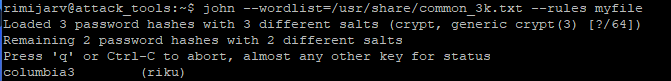
\includegraphics{riku.png}

Hashcat: \\
Hashcat was used to perform password cracking even though i had already found them with JTR.
With hashcat i had to figure out what hash type was used for password to determine the correct flag.
I found out that the hash type was "sha512crypt" which corresponds to flag "-m 7400".
In attack mode i figured that attack mode 'Straight' corresponds to flag "-a 0", which means basic attack.
With all this information i could form the command for hashcat:
\begin{verbatim}
	hashcat -m 7400 -a 0 myfile /usr/share/common_3k.txt -r /usr/share/hashcat/rules/best64.rule --force
\end{verbatim}
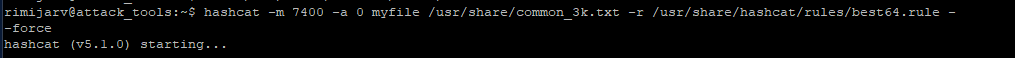
\includegraphics{start_hash.png}
which resulted in finding the same passwords as with JTR, "airborne" and "columbia3". \\
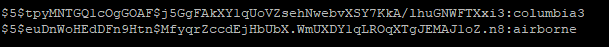
\includegraphics{hashcat.png}

\subsubsection{Verdict} \label{solution: issue-3}
Overall both tools were effective in cracking the passwords, with hashcat being slightly faster in cracking the passwords.
JTR cause some headache to figure out what to do but once i got the hang of it, it was pretty straightforward to use.
That also helped with understanding how hashcat works.

\newpage
% endregion

% region domain 2
\section{Subdomain 2}
\textbf{Platform}: TIM environment\\
\textbf{Server IP address}: 193.167.189.112

\subsection{RSA key-cracking} \label{ss: issue-2}
In this exercise i was tasked to crack an RSA key pair, which is a common cryptographic method used for secure communication.
The goal was to identify the "factors" associated with the given public key file.

Exercise was performed in private environment using TIM platform, and the key pair was provided in a 
file named "pub.pem".

\subsubsection{Minimal proof of concept}
Firstly locate the pem file, in this case pub.pem file was located in /home/rimijarv/rsa/ directory.

Public key was coded in base64, for this we need to use openssl rsa to reveal the modulus. Openssl rsa
has a flag "-pubin" which indicates that the input file has the public key. To select the file we use flag
"-in". Lastly for human readable output we need to use flag -"text". With all this information we can form the command:
\begin{verbatim}
	openssl rsa -in pub.pem -pubin -text
\end{verbatim} 
pub.pem was located in the same directory as the command was executed, so no need to specify the path.
The reveled modulus was: \\
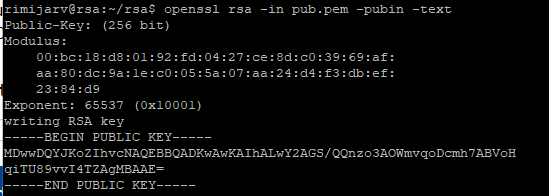
\includegraphics{openssl.png} \\
With the revealed information we need to convert modulus (hex) to base10. With this we need to understand
that modulus was in hexadecimal format, which means that it is base16. Remember to remove ":". 
To convert it to base10 we can use python:
\begin{verbatim}
	python3 -c "print(int('00bc18d80192fd0427ce8dc03969afaa80dc9a1ec0055a07aa24d4f3dbef2384d9', 16))"
\end{verbatim}
which resulted in the following base10 number:
\begin{verbatim}
	85078710682859295091507409553095548352098481513760243430344420876980368671961
\end{verbatim}
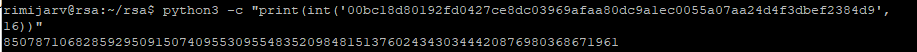
\includegraphics{python.png} \\
With the base10 number we needed to figure out what the factors were. For this we were given an tool called
msieve. Msieve was extremely easy to use where you just needed to:
\begin{verbatim}
	msieve -v 85078710682859295091507409553095548352098481513760243430344420876980368671961
\end{verbatim}
Parameter being the base10 number we got from the previous step.
which resulted in the following factors:
\begin{verbatim}
	p39 factor: 256685714581489668977306825067425055347
	p39 factor: 331450898315766891287300607911209823363
\end{verbatim}
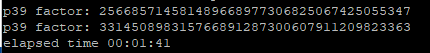
\includegraphics{factors.png} 

\newpage
% endregion

% region domain 3
\section{Subdomain 3}
\textbf{Platform}: TIM environment\\
\textbf{Server IP address}: 193.167.189.112

\subsection{RSA file-message decryption} \label{ss: issue-3}
In this exercise i was tasked to decrypt a message and return that message. Task was continous from the previous exercise,
which results i could use to help decrypting the message. The end goal was to identify the decrypted message.

Task was performed in private environment using TIM platform, and the encrypted message was provided in a file named
"encrypted\_flag.rsa".

\subsubsection{Minimal proof of concept}
To construct the private key used to decrypt the message, i needed to figure out what the python script did.
The script was used to generate the private key and i could utilize the factors obtained from the previous exercise as the
'pub.pem' file was the same. I also needed to save the private key into a .pem file so i can use it later. Filed was called
"key.pem".
With this information i could run the script with given parameters
\begin{verbatim}
	python3 reconstruct_privkey.py <pem file> <P factor> <Q factor>
	P factor: 256685714581489668977306825067425055347
	Q factor: 331450898315766891287300607911209823363
	pem file: pub.pem

	python3 reconstruct_privkey.py pub.pem 256685714581489668977306825067425055347 
	331450898315766891287300607911209823363 > key.pem
\end{verbatim}
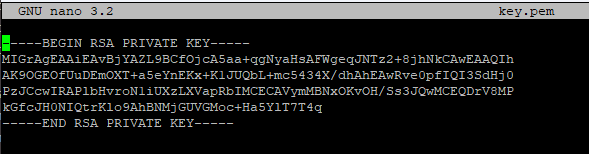
\includegraphics{pem_key.png} \\ \\
With this given constructed private key, i could use openssl to decrypt the message. 
For this i needed to use openssl rsautl and i needed to specify the correct flags for the command. --Help gave alot of useful information
about the flags which i managed to utilize to form the command:
\begin{verbatim}
	-decrypt: indicates that the operation to be performed is decryption.
	-in: specifies the input file containing the message to be decrypted (encrypted_flag.rsa).
	-inkey: specifies the file containing the private key to be used for decryption (key.pem).
	-out: specifies the output file where the decrypted message will be saved.

	openssl rsautl -decrypt -in encrypted_flag.rsa -inkey key.pem -out flag.txt
\end{verbatim}
which resulted in the decrypted message being saved in "flag.txt" file. The found flag was:
\begin{verbatim}
	FLAG=3029ab45d444c4c
\end{verbatim}
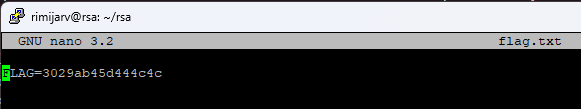
\includegraphics{flag_rsa.png}
% endregion

% region domain 4
\section{Subdomain 4}
\textbf{Platform}: TIM environment\\
\textbf{Server IP address}: 193.167.189.112

\subsection{RSA file-message forged signature} \label{ss: issue-4}
In this exercise i was tasked to forge a digital signature from given private key. Task was continous 
from the previous exercises (2, 3), which results i could use to solve the given exercise.
Task utilizes all the learned knowledge from the previous exercises.

Task was performed in private environment using TIM platform.

\subsubsection{Minimal proof of concept}
To start the exercise i needed to create a private key file, which i had done before in the previous exercise.
\begin{verbatim}
	python3 reconstruct_privkey.py <pem file> <P factor> <Q factor>
	python3 reconstruct_privkey.py pub.pem 256685714581489668977306825067425055347 331450898315766891287300607911209823363 > key.pem
\end{verbatim}
With the private key created, i can start creating a digital signature. For doing this i need to use openssl rsautl again,
but this time with different flags.
\begin{verbatim}
	-sign: indicates that the operation to be performed is signing.
	-in: specifies the input file containing the message to be signed (SIGN_THIS.txt).
	-inkey: specifies the file containing the private key to be used for signing (key.pem).
	-out: specifies the output file where the generated signature will be saved (signature.dat).

	openssl rsautl -sign -in SIGN_THIS.txt -inkey key.pem -out signature.dat
\end{verbatim}
To validate that the signature was forged i needed to check the signature file with cat and see if it had content. Alternatively
i could have used some hexdump tool to check the content.
\\
To verify the signature, i used openssl rsautl again and had to figure out the correct flags for this.
The public key file was already given in the exercise so there was no need to create it.
\begin{verbatim}
	-verify: indicates that the operation to be performed is signature verification.
	-in: specifies the input file containing the signature to be verified (signature.dat).
	-inkey: specifies the file containing the public key to be used for verification (pub.pem).
	-pubin: indicates that the input key is a public key.

	openssl rsautl -verify -pubin -inkey pub.pem -in signature.dat
\end{verbatim}
Which resulted in: SIGN=6bd6e0dd002388d
\\
To return the signature in the correct format, i had to figure out how to do it with rsautl. With the given help i 
managed to figure out the following command:
\begin{verbatim}
	-sign indicates that the operation to be performed is signing.
	-inkey specifies the file containing the private key to be used for signing (key.pem).
	-in specifies the input file containing the message to be signed (SIGN_THIS.txt).
	-hexdump indicates that the output should be displayed in hexadecimal format.
	> flag.txt to specify where the output should be saved.

	openssl rsautl -sign -inkey private_key.pem -in SIGN_THIS.txt -hexdump > flag.txt
\end{verbatim}
With this i can see the hexadump of the signature and give the result. The found signature was:
\begin{verbatim}
	0000 - 75 c3 57 d1 93 f5 53 16-c7 65 fc 51 cf 1d b4 7d   u.W...S..e.Q...
	0010 - 61 e5 37 a8 4c 6c a9 52-b6 e8 41 51 38 a9 1e d8   a.7.Ll.R..AQ8...
\end{verbatim}
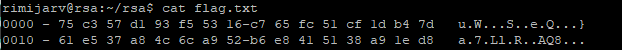
\includegraphics{rsa_hexadump.png}
\\
And with this i could form the end result for the exercise:
	75 c3 57 d1 93 f5 53 16-c7 65 fc 51 cf 1d b4 7d 61 e5 37 a8 4c 6c a9 52-b6 e8 41 51 38 a9 1e d8
% endregion